\documentclass{article}
\usepackage{amsmath}
\usepackage{amssymb}
\usepackage{graphicx}
\usepackage{hyperref}
\usepackage[version=4]{mhchem}


\begin{document}
In \(\triangle A B C, \angle B A D=30^{\circ} . \angle B A C=120^{\circ} . D\) is the midpoint of \(B C\). Prove: \(A B=2 A C\).

Solution:
\begin{center}
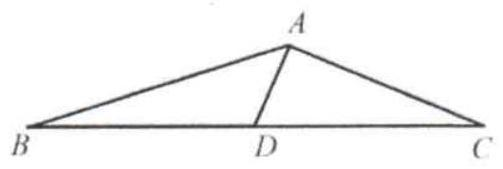
\includegraphics[width=\textwidth]{images/024(4).jpg}
\end{center}

Extend \(A D\) to \(E\) such that \(A D=D E\). Connect \(B E\).

Since \(D E=A D, \angle B D E=\angle C D A . B D=D C\).\\
Thus \(\triangle B D E \cong \triangle C D A, B E=A C\), and \(\angle E=\angle D A C\).\\
\centering
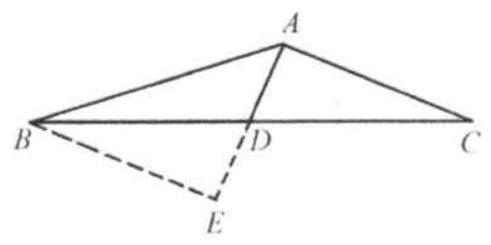
\includegraphics[width=\textwidth]{images/024.jpg}

Since \(\angle B A C=120^{\circ}, \angle B A D=30^{\circ}, \angle D A C=\angle B A C-\angle B A D=90^{\circ}\).\\
Thus, \(\angle E=90^{\circ}\).\\
Since \(\angle B A D=30^{\circ}, A B=2 A C\).


\end{document}
